\documentclass{standalone}
\usepackage{tikz}
\usetikzlibrary{fit,shapes,positioning,backgrounds}

\begin{document}

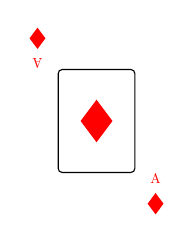
\begin{tikzpicture}[node distance=1.6cm, scale=0.5, shape aspect=0.75, fill=red]
    \node[diamond, fill, scale=0.5] (D1) at (-1.5cm,2.1cm) {};
    \node[above=0.5mm of D1, red,scale=0.5, rotate around={180:(D1)}] {A};
    \node[diamond, fill, scale=0.5] (D2) at (1.5cm,-2.1cm) {};
    \node[above=0.5mm of D2, red,scale=0.5] {A};
    \node[diamond, fill] (D3) at (0,0) {};
    \begin{pgfonlayer}{background}
        \node[draw, fill=white, rounded corners=0.5mm, fit=(D1) (D2),scale=0.5] {};
    \end{pgfonlayer}
\end{tikzpicture}

\end{document}